\documentclass[11pt, a4paper, english]{book}

\usepackage{unir}

\usepackage{caption}
\usepackage{eso-pic}
\usepackage{float}
\usepackage{graphicx}
\usepackage{natbib}
\usepackage{picture}
\usepackage{subcaption}

% Bibliography style
\bibliographystyle{abbrvnat}
\setcitestyle{authoryear,open={(},close={)}}

\setlength{\headheight}{15pt}

%---------------------------
% Título del trabajo y autor
%---------------------------
\title{Open Clusters Characterization in Gaia DR2 Using ML Algorithms}
\author{Carlos David Álvaro Yunta}
\date{13 de Septiembre de 2020}
\director{César Augusto Guzmán Álvarez}
\nombreciudad{Madrid, Spain}

%---------------------------
%marges
%---------------------------
%\usepackage[margin=1.9cm]{geometry}
%---------------------------
%---------------------------
%---------------------------
%---------------------------
\begin{document}
%\renewcommand{\listfigurename}{Índice de Ilustraciones}
%\renewcommand{\listtablename}{Índice de Tablas}
%\renewcommand{\contentsname}{Índice de Contenidos}
%\renewcommand{\figurename}{Figura}
%\renewcommand{\tablename}{Tabla}

\maketitle

\frontmatter
\tableofcontents
\listoffigures
\listoftables

\chapter{Abstract}

{\bf Nota:} En este apartado se introducirá un breve resumen en inglés del trabajo realizado (extensión máxima: 150 palabras).
Este resumen debe incluir el objetivo o propósito de la investigación, la metodología, los resultados y las conclusiones.

\medskip

{\bf Key words.} open clusters detection --- machine learning --- gaia dr2 --- data analysis

\chapter{Resumen}

{\bf Nota:} En este apartado se introducirá un breve resumen en español del trabajo realizado (extensión máxima: 150 palabras).
Este resumen debe incluir el objetivo o propósito de la investigación, la metodología, los resultados y las conclusiones.

\medskip

{\bf Palabras Clave:} detección de cúmulos abiertos --- inteligencia artificial --- gaia dr2 --- análisis de datos

\mainmatter
\chapter{Introduction}

Stellar open clusters (OC) are groups of stars gravitationally bound originated from a single molecular gas cloud.
Thus they share the same chemical composition and age, and they have similar relative positions and proper motion.
These astronomical objects are of fundamental importance to understand the spiral structure,
the dynamics and the chemical evolution of our galaxy.

Although most stars in the Milky Way are presented isolated, it is considered that most of them (or even all)
are formed in clustered environments and spend a period of time gravitationally bound with their siblings embedded
in their original molecular cloud
\cite[]{clarke2000theformationofstellarclusters} \cite[]{portegies2010young}.
The evolution of these systems tends to sparse them in a few million years by interacting gravitationally with other systems.
Galactic tidal forces and mechanisms that involves the gas loss driven by stellar feedback are other causes of disruption
\cite[]{brinkmann2017bound}.
Nevertheless, a small fraction of these systems will survive in the initial state and persist bound in bigger timescales.

Young OC allow us to research stars formation regions and improve our understanding about the mechanisms that create those stars.
On the other side, older OC give us information about stellar processes and how the galactic disk evolves.
Some highly disturbed orbits could also provide evidence of recent merge events and accretion traces from outside the galaxy
\cite[]{cantat2016abundances}.

The study of OC has been pushed forward thanks to the huge and precise dataset from the Gaia mission
\cite[]{collaboration2016description} Gaia DR2 \cite[]{gaia2018gaia}, available since 2018.
This dataset has helped to review already known open clusters and to find new ones.

\chapter{Context and State of the Art}

An initial approach to find OC is the search of overdensities along the galactic disk. In general, this is the initial point,
but even it looks simple, it presents a fundamental problem. The near field around the OC is fulled by two differenciated
kind of stars populations: the ones which belong to the OC (from a tens or hundreds to a few thousand) and a background composed
by thousands or millions of stars which don't belong to the OC. Find out which stars belong to the first group is the problem
treated in this work. This selection is crucial to properly characterize the fundamental properties of the cluster
(dynamics, total mass, age, chemical composition, etc.).

Sometimes, this problem is easy to solve by looking into astrometric parameters, such as the analysis of proper motion of those
stars belonging to the overdensity field.

\begin{figure}[htbp]
  \centering
  \begin{subfigure}[t]{0.45\textwidth}
    \centering
    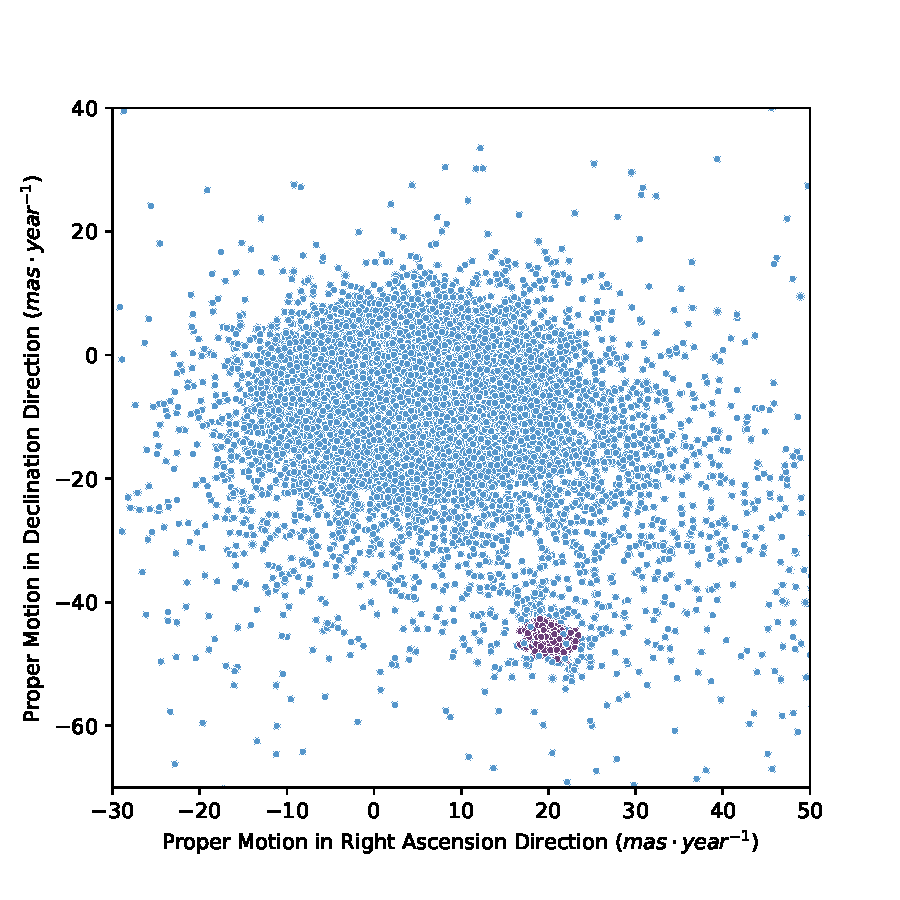
\includegraphics[width=\textwidth]{../figures/pm_melotte_22.pdf}
    \caption{Proper motions}
    \label{fig:pm_melotte_22}
  \end{subfigure}
  \hfill
  \begin{subfigure}[t]{0.45\textwidth}
    \centering
    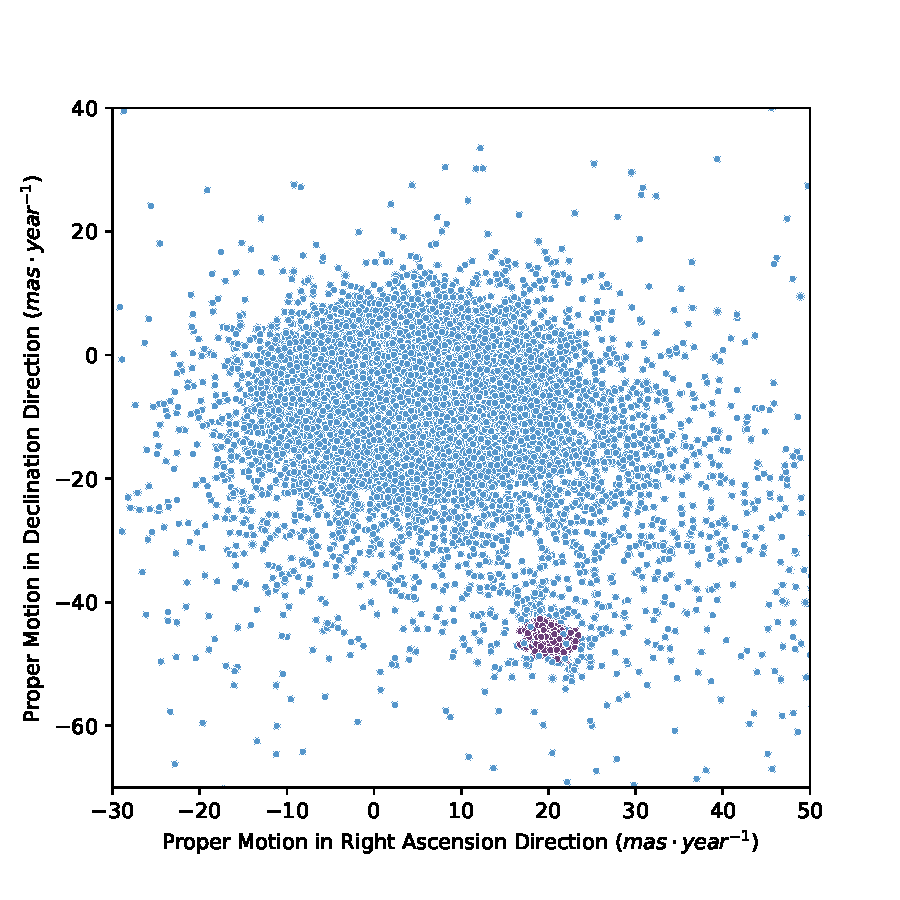
\includegraphics[width=\textwidth]{../figures/pm_melotte_22.pdf}
    \caption{Proper motions with vector lines}
    \label{fig:pm_vec_melotte_22}
  \end{subfigure}
  \caption{Open Cluster Melotte 22 (M45)}
\end{figure}

However, in general it is not as easy and becomes necessary to take into account other parameters such as distances, or even
metallicity and age (derived from isochrone curves) and requires photometric data from stars in the studied field.

\begin{figure}[htbp]
  \centering
  \begin{subfigure}[t]{0.45\textwidth}
    \centering
    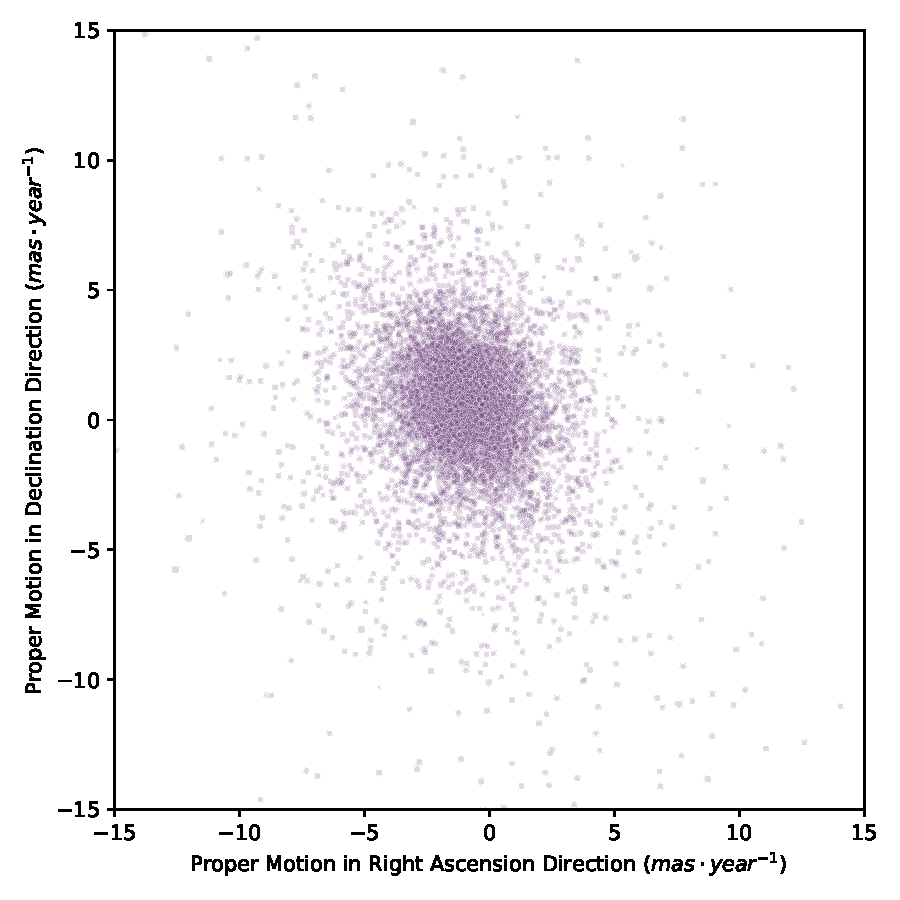
\includegraphics[width=\textwidth]{../figures/pm_ngc_2353.pdf}
    \caption{Proper motions}
    \label{fig:pm_ngc_2353}
  \end{subfigure}
  \hfill
  \begin{subfigure}[t]{0.45\textwidth}
    \centering
    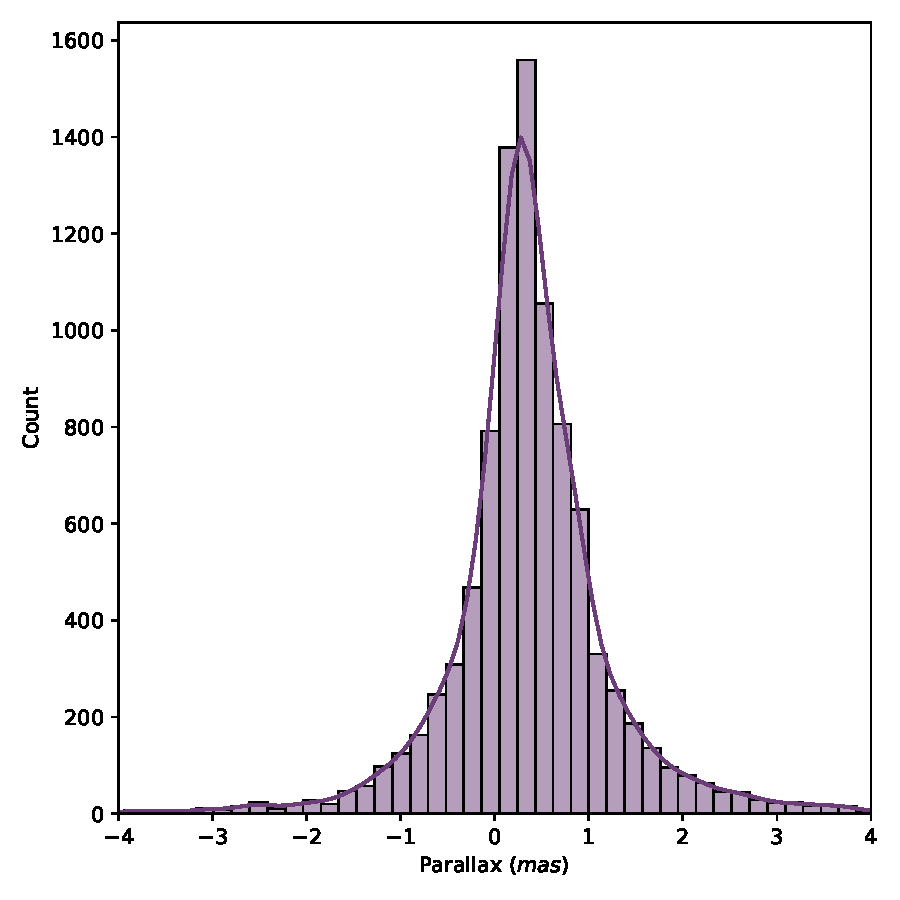
\includegraphics[width=\textwidth]{../figures/parallax_ngc_2353.pdf}
    \caption{Parallax histogram}
    \label{fig:parallax_ngc_2353}
  \end{subfigure}
  \caption{Open Cluster NGC 2353}
\end{figure}

At this point, it looks reasonable that the study of each individual cluster requires its own parametrization and technique
to identify it.

With Gaia DR2, which contains great quality astrometrical and photometric data for a huge number of stars,
a new opportunity to simplify and optimize this processes is presented.
In this context new approaches are being developed to improve current detection methods and automate the OC characterization.
This work tries to take the best from \emph{Clusterix 2.0. A Virtual Observatory tool to estimate cluster membership probability}
\cite[]{balaguer2020clusterix} and \emph{Hunting for open clusters in Gaia DR2: 582 new open clusters
in the Galactic disc} \cite[]{castro2020hunting}, and merge them into a single \emph{machine learning}
tool capable of finding open clusters eficiently without requiring powerful machines to perform the computations.

The first one is a non-parametrized method. It determines empirically the frequency functions asociated to astrometrical variables
without making any assumption about their profiles. However, it heavily does depend on the initial field selection and other
parameters related to frequency functions. \emph{Clusterix 2.0.} is presented as a web app tool inside the Spanish Virtual Observatory
(VO) framework and works together with other VO tool such as:
\emph{TOPCAT} \cite[][\url{http://www.starlink.ac.uk/topcat/}]{taylor2005topcat},
\emph{Aladin} \cite[][\url{https://aladin.u-strasbg.fr/aladin.gml}]{bonnarel2000aladin},
\emph{VOSA} \cite[][\url{http://svo2.cab.inta-csic.es/theory/vosa/}]{bayo2008vosa}, etc.

The second tool is based on Big Data techniques. Its purpose is to analyze the whole Gaia DR2 dataset looking for OCs by using
machine learning algorithms divided in two stages. In the first stage, the algorithm looks for posible OC candidates by searching
overdensities in the galactic disc.
The second stage studies candidates found in the first one by generating images with H-R diagrams and passing them
as sources to an Artificial Neural Network (ANN) which identifies isochrone patterns in photometric data (color and magnitude).
Before this approach was put into practice there were 1200 OCs known. Now, this number has been increased up to more than 2000 OCs
available at the Vizier catalogue \cite[][\url{https://vizier.unistra.fr}]{ochsenbein2000vizier}.

The method developed in this project takes as base the approach made by \citeauthor{castro2020hunting} but rapidly diverges.
In first place, performance has been taken into account since the begining, trying to get a reliable method without compromising the
needs of supercomputers.
To achieve this, instead of blindly analyzing the whole galactic disk a fields selection is made focusing in those regions with known OCs.
Then, these fields are analyzed with an homogeneous methodology based on machine learning algorithms using as sources astrometric and
photometric variables. The goal is the characterization of each individual star in the cluster, discerning wether the star belongs the OC
or not.

Thus, the main goal of this project is not the discovery of new open clusters or even candidates, but the development of a model that,
applied to already knonw open clusters, allows us the characterization of those OCs on an unsupervised way, with a reasonable computing
power and taking into account the same selection of astrometric and photometric variables for every OC.

\chapter{Requirements Description}

\chapter{Aims}

The goal of this work is to \emph{achieve a viable model for open cluster characterization based on machine learning techniques}
such as clustering algorithms and artificial neural networks.
This model must be a non-supervised non-parameterized algorithm valid for any selected OC.

The OpenClust catalogue \cite[]{dias2002new} has been used to make a preselection of sky regions for the Gaia DR2 data download.
This download is not limited to the sized registered in the catalogue. Instead, a wider region is downloaded for each cluster to include
stars from outside the cluster and take them into account when training the model so the model will be able to take apart those outsiders
when characterizing a non known cluster.

\begin{figure}[htbp]
  \centering
  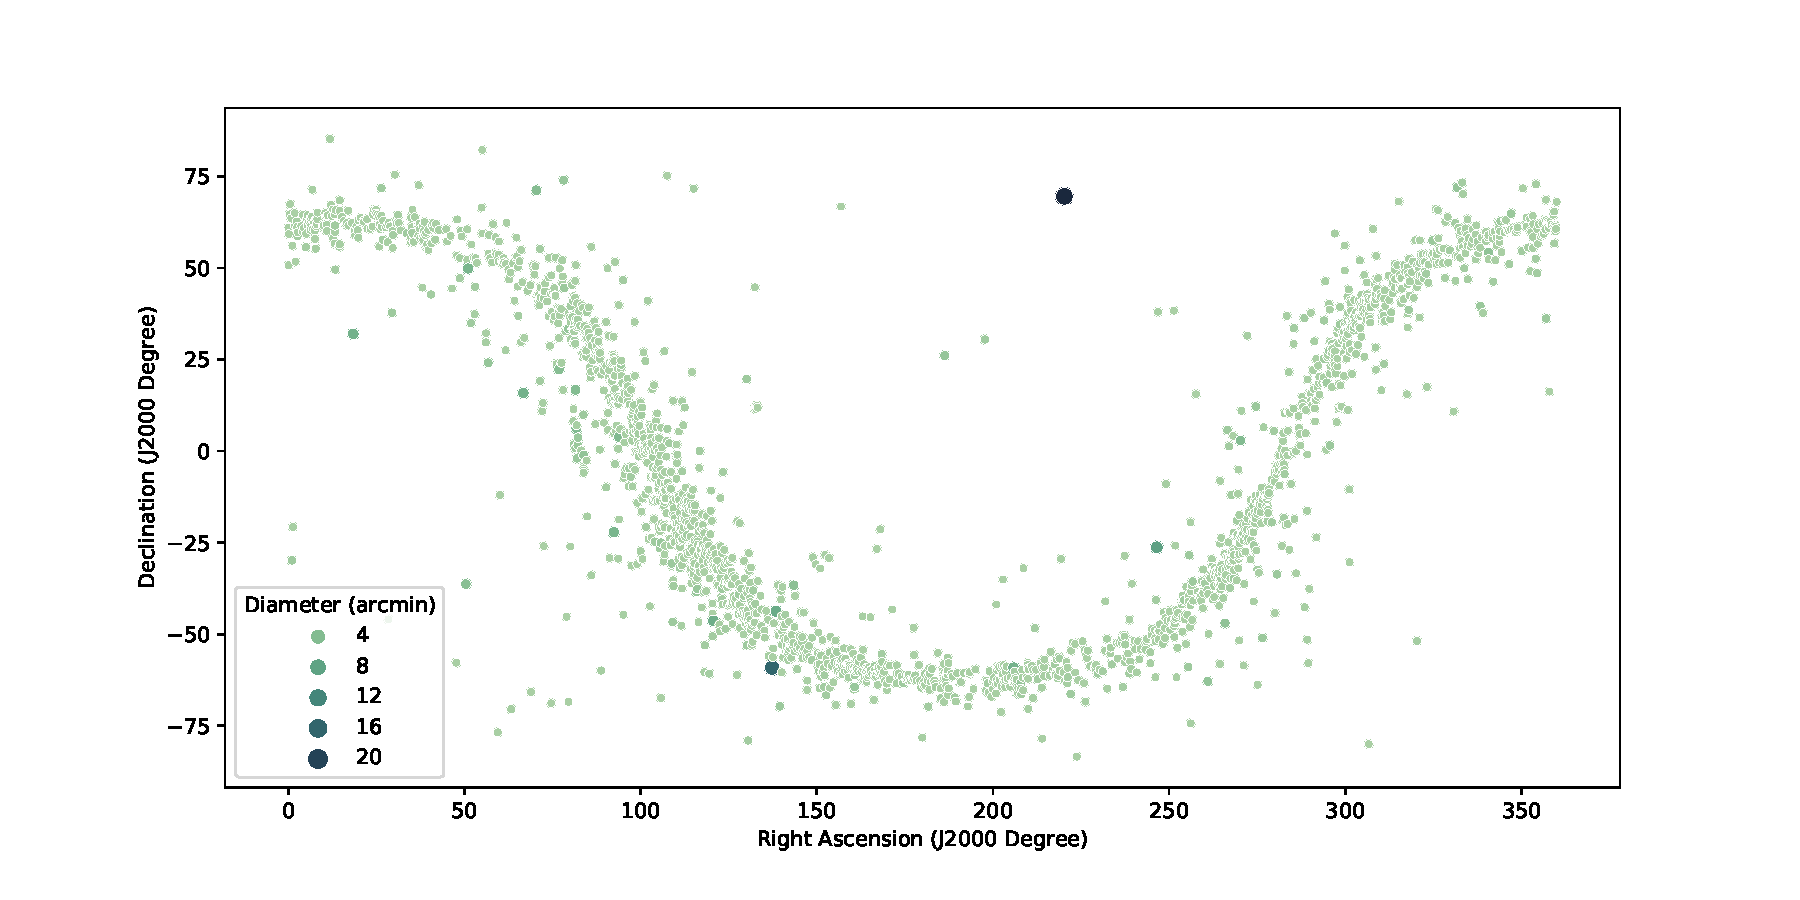
\includegraphics[width=\columnwidth]{../figures/openclust_catalogue.pdf}
  \caption{OpenClust Catalogue Distribution}
\end{figure}

A later filter will be applied to select only those OCs that fulfil one or more of the following criteria:

\begin{itemize}
  \item Cluster diameter above 25.0 arcmin
  \item Number of stars in the selected region above 40,000 stars
\end{itemize}

The final downloaded set covers nearly 60 million stars, which is significantly smaller than the whole Gaia DR2 dataset which contains
information for around 1,600 million stars.
This restriction responds to a commitment to the project delivery dates and the available computing power,
and to having a good basis for the correct model training. As an extension of this work, the trained model could be applied to a region
not covered by this preselection for a later understanding of the results.

The intention is to get a reliable and efficient non-parameterized neither supervised model over those parameterized or supervised ones.
To measure the reliability of the resulting model comparisons with other VO tools will be made.

The role for the ANN will be validating cluster members based on dynamincs and photometric data.

These are te variables to be considered in this work:

\begin{itemize}
  \item OCs and stars \emph{right ascension}: $\alpha$ and \emph{declination}: $\delta$
  \item OCs \emph{estimated sizes}: $r$
  \item \emph{Proper motion}: $\mu_{\alpha}$, $\mu_{\delta}$ and \emph{parallax}: $\varpi$
  \item \emph{Photometric}: $E(B-R)$, $G_{mag}$
  \item \emph{Radial velocity}: $RV$
  \item \emph{Associated errors} will be taken into account to estimate prediction errors
\end{itemize}

Initially, no filter will be applied over parallax neither magnitude values to the selected objects from Gaia DR2.

\chapter{Work Development}

\chapter{Conclusions and Future Work}

\chapter*{Acknowledgement}
\addcontentsline{toc}{chapter}{Acknowledgement}

This work has made use of data from the European Space Agency (ESA) mission
{\it Gaia} (\url{https://www.cosmos.esa.int/gaia}), processed by the {\it Gaia}
Data Processing and Analysis Consortium (DPAC,
\url{https://www.cosmos.esa.int/web/gaia/dpac/consortium}). Funding for the DPAC
has been provided by national institutions, in particular the institutions
participating in the {\it Gaia} Multilateral Agreement.

\medskip

This publication makes use of VOSA, developed under the Spanish Virtual Observatory project
supported by the Spanish MINECO through grant AyA2017-84089.
VOSA has been partially updated by using funding from the European Union's Horizon 2020 Research
and Innovation Programme, under Grant Agreement nº 776403 (EXOPLANETS-A)

\medskip

This research has made use of the VizieR catalogue access tool, CDS, Strasbourg, France (DOI : 10.26093/cds/vizier).
The original description of the VizieR service was published in 2000, \cite[A\&AS 143, 23]{ochsenbein2000vizier}

\bibliography{references}
\addcontentsline{toc}{chapter}{Bibliography}

\AddToShipoutPicture*{
  \AtPageLowerLeft{
    \makebox(\paperwidth,0)[rb]{
      
\includegraphics[width=4cm,height=4cm,keepaspectratio]{../figures/github_qr.pdf}
    }
  }
}

\appendix
\chapter{Appendix}

%\includepdf[pages=-]{anexo.pdf} # TODO: Descomentar cuando el artículo esté hecho
\end{document}
